\documentclass{article}

% External references
\usepackage{pgf}
\usepackage{tikz}
\usepackage{amsmath}
\usepackage{amssymb}
\usepackage{amsthm}
\usepackage{IEEEtrantools}
\usepackage{mathrsfs}

% For the Markov chain diagrams
\usetikzlibrary{arrows,automata}

\title{von Foerster Hazard Rate Models}
\begin{document}
  \pagenumbering{gobble}
  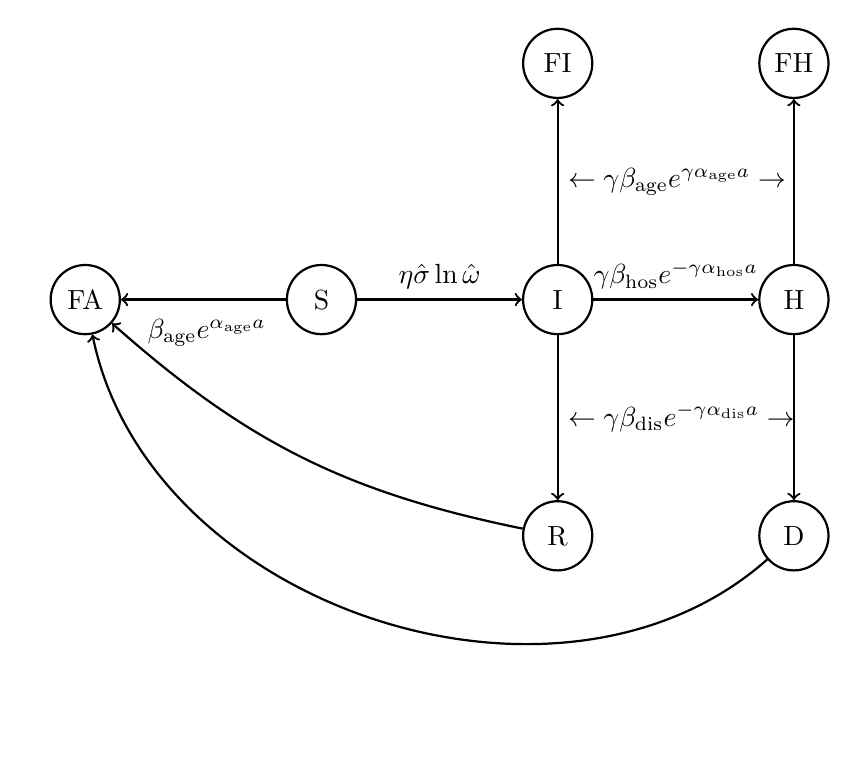
\begin{tikzpicture}[->,thick,node distance=3cm]
    \node[state] (FA)               {FA};
    \node[state] (S)  [right of=FA] {S};
    \node[state] (I)  [right of=S]  {I};
    \node[state] (H)  [right of=I]  {H};
    \node[state] (R)  [below of=I]  {R};
    \node[state] (D)  [below of=H]  {D};
    \node[state] (FI) [above of=I]  {FI};
    \node[state] (FH) [above of=H]  {FH};
    \path
      (S) edge (FA)
      (S) edge node [above] {$\eta\hat{\sigma} \ln\hat{\omega}$} (I)
      (I) edge node [above] {$\gamma\beta_\text{hos} e^{-\gamma\alpha_\text{hos} a}$} (H)
      (I) edge node [right] {$\leftarrow\gamma\beta_\text{dis} e^{-\gamma\alpha_\text{dis} a}\rightarrow$} (R)
      (H) edge (D)
      (I) edge node [right] {$\leftarrow\gamma\beta_\text{age} e^{\gamma\alpha_\text{age} a}\rightarrow$} (FI)
      (H) edge (FH)
      (R) edge [bend left=15] node [above, pos=0.9] {$\qquad\qquad\beta_\text{age} e^{\alpha_\text{age} a}$} (FA)
      (D) edge [bend left=60] (FA);
  \end{tikzpicture}
\end{document}